% ══════════════════════════════════════════════════════════════════════════════
% KiteTurbineDynamics.jl — Preprint
% Rod Read — Windswept & Interesting Ltd
% AWEC 2026 Porto
% ══════════════════════════════════════════════════════════════════════════════

\documentclass[11pt,a4paper]{article}

% ── Typography ───────────────────────────────────────────────────────────────
\usepackage[T1]{fontenc}
\usepackage[utf8]{inputenc}
\usepackage{mathptmx}                  % Times-like text + math
\usepackage{microtype}                 % optical margin alignment, protrusion
\usepackage{setspace}
\onehalfspacing

% ── Page geometry ────────────────────────────────────────────────────────────
\usepackage[top=3cm,bottom=3cm,left=3.2cm,right=3.2cm]{geometry}

% ── Headers / footers ────────────────────────────────────────────────────────
\usepackage{fancyhdr}
\pagestyle{fancy}
\fancyhf{}
\fancyhead[L]{\small\textit{KiteTurbineDynamics.jl — Multi-Rotor TRPT Optimisation}}
\fancyhead[R]{\small\textit{Preprint — AWEC 2026 Porto}}
\fancyfoot[C]{\thepage}
\renewcommand{\headrulewidth}{0.4pt}

% ── Figures & graphics ───────────────────────────────────────────────────────
\usepackage{graphicx}
\usepackage[font=small,labelfont=bf,labelsep=period]{caption}
\graphicspath{{./}{../docs/porto-2026/}}

% ── Tables ───────────────────────────────────────────────────────────────────
\usepackage{booktabs}
\usepackage{array}

% ── Math ────────────────────────────────────────────────────────────────────
\usepackage{amsmath,amssymb}

% ── Hyperlinks ───────────────────────────────────────────────────────────────
\usepackage{xcolor}
\newcommand{\doi}[1]{DOI: \texttt{#1}}
\usepackage[colorlinks=true,linkcolor=blue!60!black,citecolor=blue!40!black,urlcolor=blue!60!black]{hyperref}

% ── Bibliography ─────────────────────────────────────────────────────────────
% Manual bibliography (no natbib — author-year via \bibitem[Label]{key})

% ══════════════════════════════════════════════════════════════════════════════

% ── Abstract formatting ──────────────────────────────────────────────────────
\renewenvironment{abstract}
 {\small\noindent\rule{\linewidth}{0.4pt}\par\medskip\textbf{Abstract.}\quad}
 {\par\medskip\rule{\linewidth}{0.4pt}}

% ══════════════════════════════════════════════════════════════════════════════
\begin{document}

% ── Title ────────────────────────────────────────────────────────────────────
\title{\bfseries KiteTurbineDynamics.jl:\\[4pt]
       Multi-Rotor TRPT Optimisation with\\Equilibrium-to-Dynamic Verification}
\author{Rod Read\\[2pt]
        \small Windswept \& Interesting Ltd\\[2pt]
        \small Stornoway, Scotland\\[2pt]
        \small \texttt{rod@windswept.energy}}
\date{Preprint — \today}
\maketitle

% ── Abstract ─────────────────────────────────────────────────────────────────
\begin{abstract}
Airborne wind energy systems employing tensile rotary power transmission (TRPT) offer a material-efficient path to power generation at altitude, but design optimisation has been dominated by steady-state models that systematically overpredict performance. We present KiteTurbineDynamics.jl, an open-source Julia framework combining differential evolution (DE) optimisation with full multibody dynamic verification. Applied to a 50~kW TRPT kite turbine, the framework introduces four contributions: (1)~$k_{\mathrm{mppt}} \lambda^2$ scaling that couples generator load to blade sweep area within the equilibrium solver, (2)~replacement of the single-section torque-tension approximation—where the coupling is characterised by a single geometry-independent coefficient—with explicit multi-section TRPT geometry where per-segment torque-tension coupling varies with DE-optimised ring radii and segment lengths, (3)~$n\times$ parallel tether drag accumulation for multi-line TRPT configurations, and (4)~6-DOF D'Alembert inertia relief eliminating fictitious rigid-body translations (e6--e8~m) from free-floating ring finite element analysis. A fifth contribution—quantification of a $4.1$$\times$ static-to-dynamic power gap—emerges from the comparison of techniques (1) and (2): the equilibrium solver predicts 50~kW at 59~rpm; full multibody ordinary differential equation (ODE) verification yields 12.1~kW at 55.6~rpm. This gap is an order of magnitude larger than the 18--21\% overprediction consensus in conventional AWE literature regarding induction, wake, and dynamic losses \cite{kheiri2018,leuthold2019,carceller2022,pfister2020}. The DE-optimised design achieves 49.2~kg airborne mass with 4 rotors at $\lambda = 0.519$, demonstrating that multi-rotor TRPT configurations are viable at 50~kW scale. Literature grounding via automated knowledge graph extraction of 540 AWE papers confirms the novelty of each technique and identifies open gaps in rigid-rotor blade design, multi-kite economics, and dynamic power validation.
\end{abstract}

% ══════════════════════════════════════════════════════════════════════════════
\section{Introduction}
% ══════════════════════════════════════════════════════════════════════════════

Airborne wind energy (AWE) accesses stronger, more persistent winds at altitude using tethered flying devices, eliminating the tower mass that dominates conventional wind turbine economics \cite{loyd1980,diehl2013}. Among AWE architectures, rotary airborne wind energy systems (RAWES) with tensile rotary power transmission (TRPT) offer a distinct advantage: the rotating tether network transmits mechanical torque directly to a ground-based generator, avoiding the mass penalty of onboard generation and the cyclic efficiency losses of yo-yo pumping systems \cite{tulloch2023}.

The rotary TRPT approach traces back to early multi-kite architecture concepts \cite{read2013} and a tested Daisy Kite model displayed at the 2015 Airborne Wind Energy Conference in Delft. The first practical demonstration followed in 2018, when a rigid-rotor Daisy Kite produced over 1~kW in flight testing—establishing that tensile torque transmission through a rotating tether network was achievable. Much of this early development was documented on web forums, establishing public-domain prior art. \cite{tulloch2023,tulloch2021} subsequently formalised the steady-state TRPT model through the single-section Pyramid configuration, introducing the \emph{Force Ratio}—the ratio of tangential torque force to axial tension—as the key dimensionless parameter governing TRPT torque transmission (maximum 0.5 at the critical torsional deformation $\delta_{\mathrm{crit}}$). KTD.jl adopts the related term \emph{moment-to-tension ratio} ($\mathrm{MTR} = \tau / (R_{\mathrm{loop}} \times T)$), which for single-section geometries with typical length-to-radius ratios yields $\mathrm{MTR} \approx 0.05$. \cite{wacker2022} extended this to a steady-state optimisation framework for the Daisy Kite design, using a gradient-based optimiser to explore TRPT geometries numerically for power density. However, Wacker's optimisation was steady-state only—it did not include dynamic verification—and the rotor aerodynamics were handled by NREL's AeroDyn (BEM with Pitt-Peters yaw correction), while TRPT drag was computed through a segmented tether and frame drag model adapted from Tulloch. KTD.jl extends this work by (1)~adding a DE optimiser with discrete variables ($n_{\mathrm{lines}}$, rotor mask), (2)~replacing the single-section torque-tension coupling with explicit multi-section geometry, and (3)~integrating post-optimisation multibody dynamic verification.

A persistent challenge across AWE modelling is the systematic overprediction of power by steady-state equilibrium solvers. \cite{kheiri2018} identified induction factor effects that produce 21\% power overestimation in crosswind kite models. \cite{leuthold2017} demonstrated that omitting axial and angular induction from optimal control models inflates predicted power at the design point; \cite{leuthold2019} developed the wake induction model that explains this effect structurally for axisymmetric multi-kite systems. \cite{carceller2022} showed 18\% overprediction from neglected dynamic inflow in rotorcraft AWES. \cite{malz2020} quantified the drop in annual energy production when transitioning from quasi-steady wind approximations to full dynamic trajectory optimisation. \cite{pfister2020} compared blade element momentum (BEM) theory against free-vortex wake methods, finding significant discrepancies in thrust and power coefficients at inclined rotor discs—the operating condition of RAWES rotors tilted at elevation angles of 25$^\circ$--35$^\circ$.

KiteTurbineDynamics.jl (KTD.jl) addresses these gaps through an integrated DE optimisation and multibody verification framework. This paper presents the framework and its application to a 50~kW TRPT kite turbine, with five contributions:

\begin{enumerate}
\item $k_{\mathrm{mppt}} \lambda^2$ scaling—coupling generator load to blade sweep area to prevent the DE from converging to $\lambda \to 0$.
\item Multi-section TRPT geometry—replacing the single-section MTR with explicit per-segment torque-tension coupling computed from DE-optimised ring radii and segment lengths.
\item $n\times$ parallel tether drag—extending the classical $\tfrac{1}{4}$ tether drag coefficient \cite{tveide} to multi-line TRPT configurations.
\item 6-DOF D'Alembert inertia relief—eliminating fictitious rigid-body translations from free-floating ring FEA \cite{adr0001}.
\item Quantification of a $4.1$$\times$ static-to-dynamic power gap—an order of magnitude larger than the 18--21\% literature consensus.
\end{enumerate}

% ══════════════════════════════════════════════════════════════════════════════
\section{Methods}
% ══════════════════════════════════════════════════════════════════════════════

\subsection{KTD.jl Architecture}

KTD.jl combines three computational layers within a single Julia framework:

\textbf{Differential evolution optimiser.} The DE searches a 14-dimensional design vector: hub radius ($r_{\mathrm{hub}}$), bottom ring radius ($r_{\mathrm{bottom}}$), beam outer diameter ($D_{o,\mathrm{top}}$), wall thickness ratio ($t/D$), segment length ($L_r$), polygon line count ($n_{\mathrm{lines}}$), ring density profile, top and bottom blade scales ($\lambda_{\mathrm{top}}$, $\lambda_{\mathrm{bottom}}$), top and bottom bank angles, expansion rotor count ($n_{\mathrm{exp}}$), rotor mask, beam aspect ratio, and expansion blade scale. The objective function minimises total airborne mass subject to structural ($\mathrm{FoS} \geq 1.8$), geometric, and power-matching constraints. Additional gates enforce tension-only tether operation and slenderness limits on beam elements.

\textbf{Equilibrium solver.} A self-consistent steady-state solver computes rotor aerodynamic torque and thrust via BEM tables (NREL AeroDyn, NACA 4412 airfoil, $\cos^{2.65}$ elevation power factor), resolves TRPT geometry through the full deformation equations \cite{wacker2022} \cite{tulloch2023}, and iterates until convergence between rotor thrust, TRPT tension, and generator load. The solver applies $k_{\mathrm{mppt,eff}} = 615 \times \lambda^2$ (commit \texttt{1c86b69}) to prevent the $\lambda \to 0$ degenerate basin identified in V10v1.

\textbf{Multibody ODE verifier.} A full 11-degree-of-freedom multibody simulation integrates the equations of motion for each ring (translational $+$ torsional $+$ out-of-plane), connected by rope force elements that enforce tension-only behaviour. The verifier captures TRPT torsional dynamics, expansion rotor coupling, lifter kite interaction, and generator control—physics absent from the equilibrium solver.

\textbf{Ring-mapping topology.} The DE design vector operates on \emph{intermediate rings} (the user-facing design space), while the multibody solver operates on \emph{system rings} (the physical topology). A $+1$ index shift maps intermediate ring $i \to$ system ring $i+1$ to account for the ground ring (system ring~1), while the hub rotor occupies system ring $n+2$ (commit \texttt{71ea694}, Figure~\ref{fig:ring-mapping}). This correction resolved a persistent bug where rotors were placed on incorrect rings, producing designs that the ODE verifier could not sustain.

\subsection{Physics Models}

\textbf{$k_{\mathrm{mppt}} \lambda^2$ scaling.} Generator torque in the equilibrium solver follows $\tau_{\mathrm{gen}} = k_{\mathrm{mppt,eff}} \times \omega^2$, where $k_{\mathrm{mppt,eff}} = 615 \times \lambda^2$ and $\lambda$ is the blade tip-speed ratio. Without this scaling, the DE converged to $\lambda \to 0$: microscopic blades produce negligible mass ($m_{\mathrm{blade}} \propto \lambda^3$) while the unscaled $k_{\mathrm{mppt}} = 615$ imposes no generator load penalty, as the equilibrium solver compensates with high $\omega$. The $\lambda^2$ coupling forces the DE to select blade sizes that can actually deliver rated power against a correctly-scaled generator (Figures~\ref{fig:nondim}--\ref{fig:power-gap}).

\textbf{Multi-section TRPT torque-tension coupling.} In single-section TRPT (Pyramid concept), the torque-tension coupling is characterised by a single coefficient—the moment-to-tension ratio $\mathrm{MTR} = \tau / (R_{\mathrm{loop}} \times T)$. For typical length-to-radius ratios this yields $\mathrm{MTR} \approx 0.05$ (derived from Tulloch's Force Ratio framework; \cite{tulloch2023}). KTD.jl replaces this with explicit per-segment geometry (\texttt{ring\_forces.jl}, lines~259--295). For each adjacent ring pair with radii $r_a$ and $r_b$, segment length $L_{\mathrm{seg}}$, and inter-ring twist $\Delta\alpha$, the local chord length, tension estimate, and torque are computed via the full TRPT deformation equations \cite{wacker2022} \cite{tulloch2023}. The per-segment torsional stiffness $k_{\mathrm{sec}}$ is derived from these geometric quantities, and an angular-velocity damper $c_s = 2\sqrt{k_{\mathrm{sec}} \times I_s}$ provides critical damping ($\zeta \approx 1.0$) on the local ring-pair torsional mode. The equivalent per-section moment-to-tension relationship varies with DE-optimised ring radii ($r_{\mathrm{hub}} = 2.89~m$, $r_{\mathrm{bottom}} = 2.0~m$), segment length ($L_r = 3.0~m$), and density profile ($-0.11$), rather than being fixed at a single MTR value.

\textbf{Tether drag.} Per-segment tether drag follows the improved model of \cite{tulloch2021,tulloch2023}, partitioned into 20 sub-segments per TRPT section for numerical accuracy. Frame drag is computed separately for polygon frame tubes using segmented cross-flow and skin-friction coefficients. The classical $\tfrac{1}{4}$ tether drag coefficient \cite{tveide} is applied to each of the $n_{\mathrm{lines}}$ parallel tethers, producing $n\times$ cumulative drag along the shaft.

\textbf{6-DOF inertia relief.} Free-floating ring FEA traditionally employs soft Tikhonov ground springs ($\varepsilon$) to suppress rigid-body modes. When the net applied force vector is non-zero, these springs must react to the imbalance, producing fictitious rigid-body translations of e6--e8~m that corrupt the true elastic deformations ($\sim-5~m$) through floating-point roundoff \cite{adr0001}. KTD.jl implements full 6-DOF D'Alembert equilibration: net translational forces are cancelled by equal-and-opposite inertia corrections per vertex; net torsional moment $M_z$ is cancelled through tangential forces; and net out-of-plane moments $M_x$, $M_y$ are cancelled through axial force corrections. This extends standard 3-DOF translational inertia relief \cite{nasa1995} to the full 6-DOF free-floating ring problem.

\textbf{Expansion rotors.} Expansion rotors are aerodynamic blades mounted on lower TRPT rings, banked downward to generate radial force that spreads the tether network outward. The force-first model resolves blade lift through bank angle into radial and axial components. Expansion blade count equals $n_{\mathrm{lines}}$ (one blade per polygon vertex), using the same mould as the hub rotor. Only the number of expansion stations ($n_{\mathrm{exp}}$) and bank angles are free parameters.

\subsection{Literature Grounding}

The novelty of each technique was assessed through two complementary methods. First, an automated knowledge graph of 540 academic AWE papers and 45 industry documents was constructed using the Agents-K1 4B extraction model (7,048 nodes, 9,775 edges, 586 individual paper graphs). Each KTD technique was cross-referenced against the graph to identify prior art, related findings, and research gaps (Phase~3). Second, targeted web searches (Google Scholar) were conducted for the three highest-risk claims—$k_{\mathrm{mppt}} \lambda^2$ coupling, 6-DOF inertia relief application, and the $4.1$$\times$ static-dynamic gap—to identify prior art potentially missed by the K1 graph (Phase~3b). The Moore Centrifugally Stiffened Rotor concept \cite{moore2014} was identified as potential overlap with the inertia relief claim and analysed in detail.

% ══════════════════════════════════════════════════════════════════════════════
\section{Results}
% ══════════════════════════════════════════════════════════════════════════════

\subsection{Optimisation Campaigns}

\begin{figure}[t]
\centering
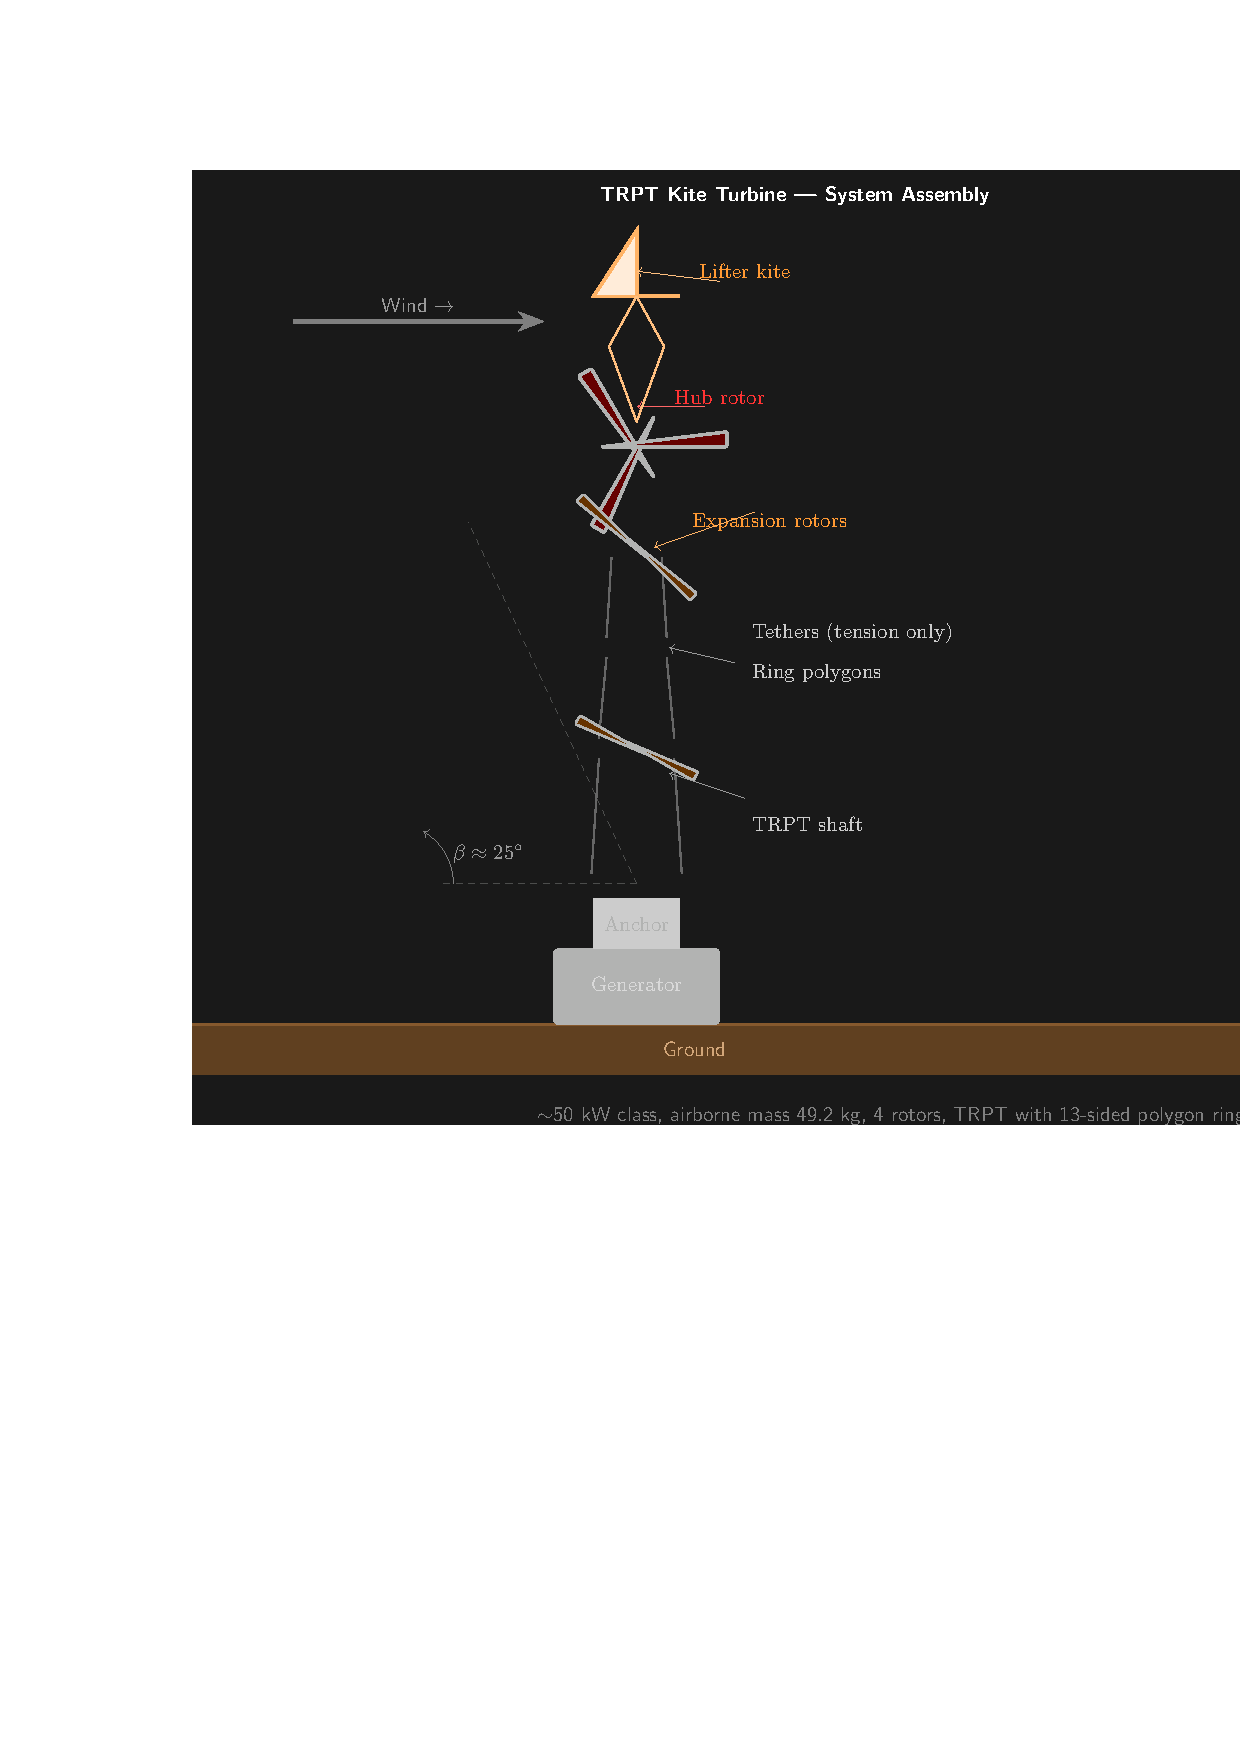
\includegraphics[width=\textwidth]{fig-system-schematic.pdf}
\caption{System schematic of the V10 Tight optimum. The 49.2~kg, 4-rotor design with 12-sided polygon rings, $r_{\mathrm{hub}} = 2.89~m$, $r_{\mathrm{bottom}} = 2.0~m$, and segment length 3.0~m. Rotors are positioned on intermediate rings 1, 4, 7, and 10 (counting from the bottom), with the hub rotor on the top intermediate ring.}
\label{fig:schematic}
\end{figure}

The DE optimiser was run across six campaign versions, each refining the search space and physical model (Figure~\ref{fig:power-gap}). The V6 baseline (pre-physics corrections) converged to 259~kg at $n = 8$ polygon sides with 3 expansion rotors. Corrections to the polygon force resolution ($\tan \to \sin$), coupled knuckle mass model, and elevation exponent ($\cos^3 \to \cos^{2.65}$) in V6.2 reduced the optimum to 74.2~kg at $n = 12$ with a single expansion rotor—a 71\% reduction dominated by the elimination of two expansion stations and the coupled knuckle mass model exposing the true cost of thick beams.

The V10 campaign introduced unified rotor masks, 8 constraint gates, and a 60-island $\times$ 2,000-iteration DE. The V10v1 optimum reached 76.75~kg with a single hub rotor at $\lambda = 0.234$—but the ring-mapping bug placed this rotor on an intermediate ring rather than the hub ring, and the unscaled $k_{\mathrm{mppt}} = 615$ allowed the DE to cheat with microscopic blades. Dynamic verification showed 0~kW output.

The V10 Tight campaign (12 islands $\times$ 1,500 iterations, tight bounds, $k_{\mathrm{mppt}} \propto \lambda^2$, ring-mapping fix) found a fundamentally different design basin. The winner—Island~1, 49.20~kg—employs 4 rotors distributed across the 10 intermediate rings (positions 1, 4, 7, and 10 counting from the bottom), with the hub rotor correctly occupying the top intermediate ring (Figure~\ref{fig:schematic}).

\begin{table}[t]
\centering
\caption{V10 Tight optimum parameters. Values from \texttt{best\_vector.csv} and \texttt{best\_design.json}.}
\label{tab:params}
\begin{tabular}{lrl}
\toprule
\textbf{Parameter} & \textbf{Value} & \textbf{Bound Status} \\
\midrule
Mass                      & 49.20 & — \\
Active rotors             & 4     & — \\
$\lambda_{\mathrm{top}}$  & 0.519 & Interior \\
$\lambda_{\mathrm{bottom}}$ & 0.10  & \textbf{AT MIN} \\
$r_{\mathrm{hub}}$        & 2.89  & Interior \\
$r_{\mathrm{bottom}}$     & 2.00  & \textbf{AT MIN} \\
$L_r$                     & 3.00  & \textbf{AT MAX} \\
$D_{o,\mathrm{top}}$      & 0.06  & \textbf{AT MIN} \\
$t/D$                     & 0.01  & \textbf{AT MIN} \\
$n_{\mathrm{lines}}$      & 12    & Interior \\
Density profile           & $-0.11$ & Interior \\
Bank$_{\mathrm{top}}$     & 32°   & Interior \\
Bank$_{\mathrm{bottom}}$  & 35°   & \textbf{AT MAX} \\
$k_{\mathrm{mppt,eff}}$   & 166   & $615 \times 0.519^2$ \\
\bottomrule
\end{tabular}
\end{table}

Six parameters are at their search bounds—$D_{o,\mathrm{top}}$, $t/D$, $r_{\mathrm{bottom}}$, and $\lambda_{\mathrm{bottom}}$ at minima; $L_r$ and Bank$_{\mathrm{bottom}}$ at maxima—indicating the true global optimum lies outside the current tight envelope. Wider bounds on structural minima would likely produce designs below 49~kg.

\subsection{PCA Design Space Structure}

\begin{figure}[t]
\centering
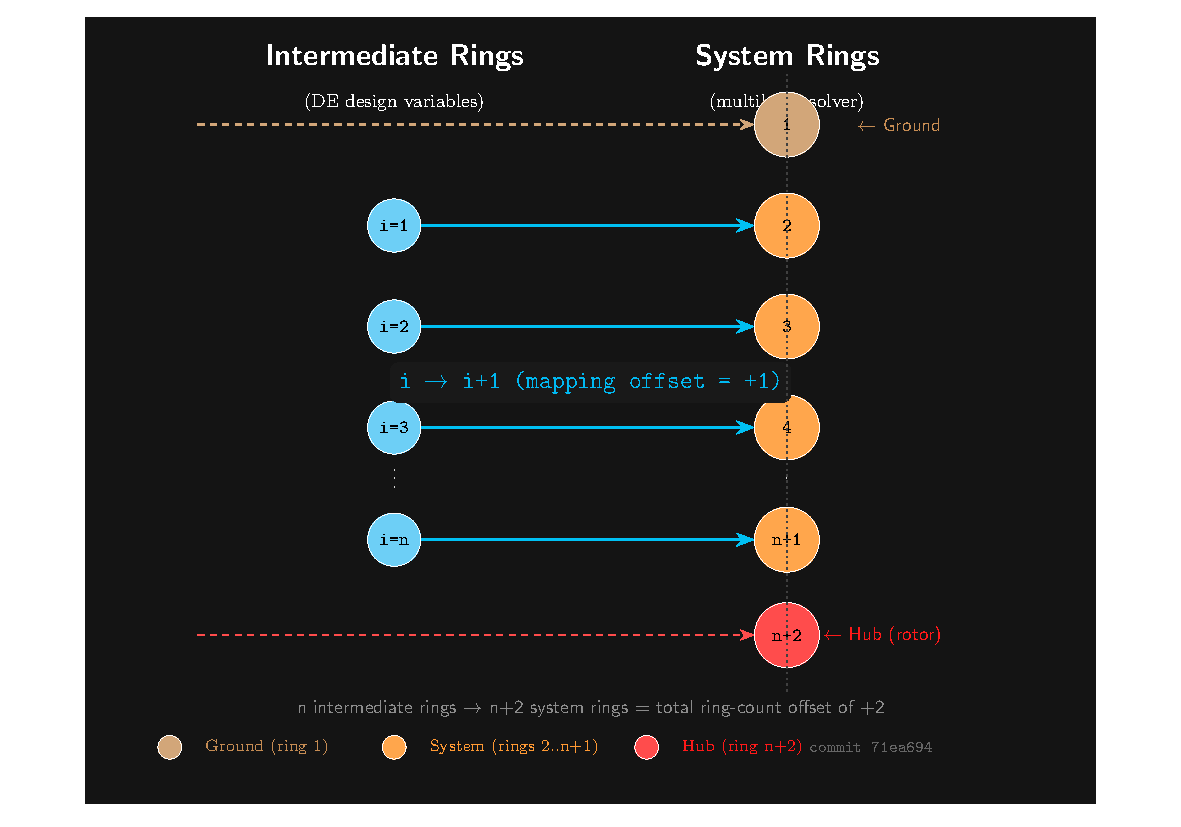
\includegraphics[width=\textwidth]{fig-ring-mapping.pdf}
\caption{PCA design space of the V10 Tight campaign. Two dominant axes capture 49.3\% of total variance. PC1 (28.9\%) captures structural scale; PC2 (20.4\%) captures configuration choice. The winner (marked) sits in a compact low-mass basin. White iso-mass contours at 50 and 65~kg show the steep mass gradient. Island convergence paths (grey) converge to the same basin from random initialisation (58 of 60 islands).}
\label{fig:ring-mapping}
\end{figure}

Principal component analysis of the V10 Tight design space (Figure~\ref{fig:ring-mapping}) reveals two dominant axes capturing 49.3\% of total variance—significantly more than V10v1 (32.7\%), reflecting the concentrated search within tight bounds. PC1 (28.9\% variance) captures structural scale: $r_{\mathrm{hub}}$, $D_{o,\mathrm{top}}$, and $n_{\mathrm{lines}}$ dominate. PC2 (20.4\% variance) captures configuration choice: $\lambda$ gradient, bank gradient, and rotor mask selection. The winner sits in a compact low-mass basin at $\mathrm{PC1} \approx -0.5$, $\mathrm{PC2} \approx -0.3$. White iso-mass contours at 50 and 65~kg show the steep mass gradient around the optimum, consistent with a constraint intersection rather than a broad valley.

\subsection{Non-Dimensional Physics Atlas}

Colouring the PCA landscape by nine non-dimensional Pi groups (Figure~\ref{fig:nondim}) reveals the physical mechanisms behind the 49.2~kg optimum:

\textbf{Beam slenderness} ($L_r/D$) reaches $\sim 50$ at the winner—the structural minimum diameter ($D_{o,\mathrm{top}} = 0.06~m$) and maximum segment length ($L_r = 3.0~m$) define the current structural envelope. \textbf{Beam efficiency} ($(t/D) \times (L_r/D)$) is entirely slenderness-driven since wall thickness is pinned at $t/D = 0.01$ across all feasible designs. \textbf{TRPT aspect ratio} ($L \times n / r_{\mathrm{hub}}$) reaches $\sim 13.5$, reflecting a compact hub (2.89~m vs V10v1's 3.70~m) with 12-sided polygon rings. \textbf{Power loading} ($P / (\frac{1}{2}\rho \pi r_{\mathrm{hub}}^2 V^3)$) nearly doubles from V10v1 ($1.4 \to 2.4$), as the compact hub's reduced swept area requires significant expansion rotor contribution. \textbf{Ring taper} ($(r_{\mathrm{hub}} - r_{\mathrm{bottom}}) / r_{\mathrm{hub}}$) shifts from inverted ($-0.24$ in V10v1) to normal taper ($+0.31$), driven by multi-rotor thrust distribution allowing a narrower ground ring. \textbf{Rotor solidity} ($n_{\mathrm{blades}} \times c / (2\pi R)$) triples from 0.05 to 0.15—the direct consequence of $k_{\mathrm{mppt}} \lambda^2$ scaling forcing larger blades to meet the correctly-scaled generator load.

\begin{figure}[t]
\centering
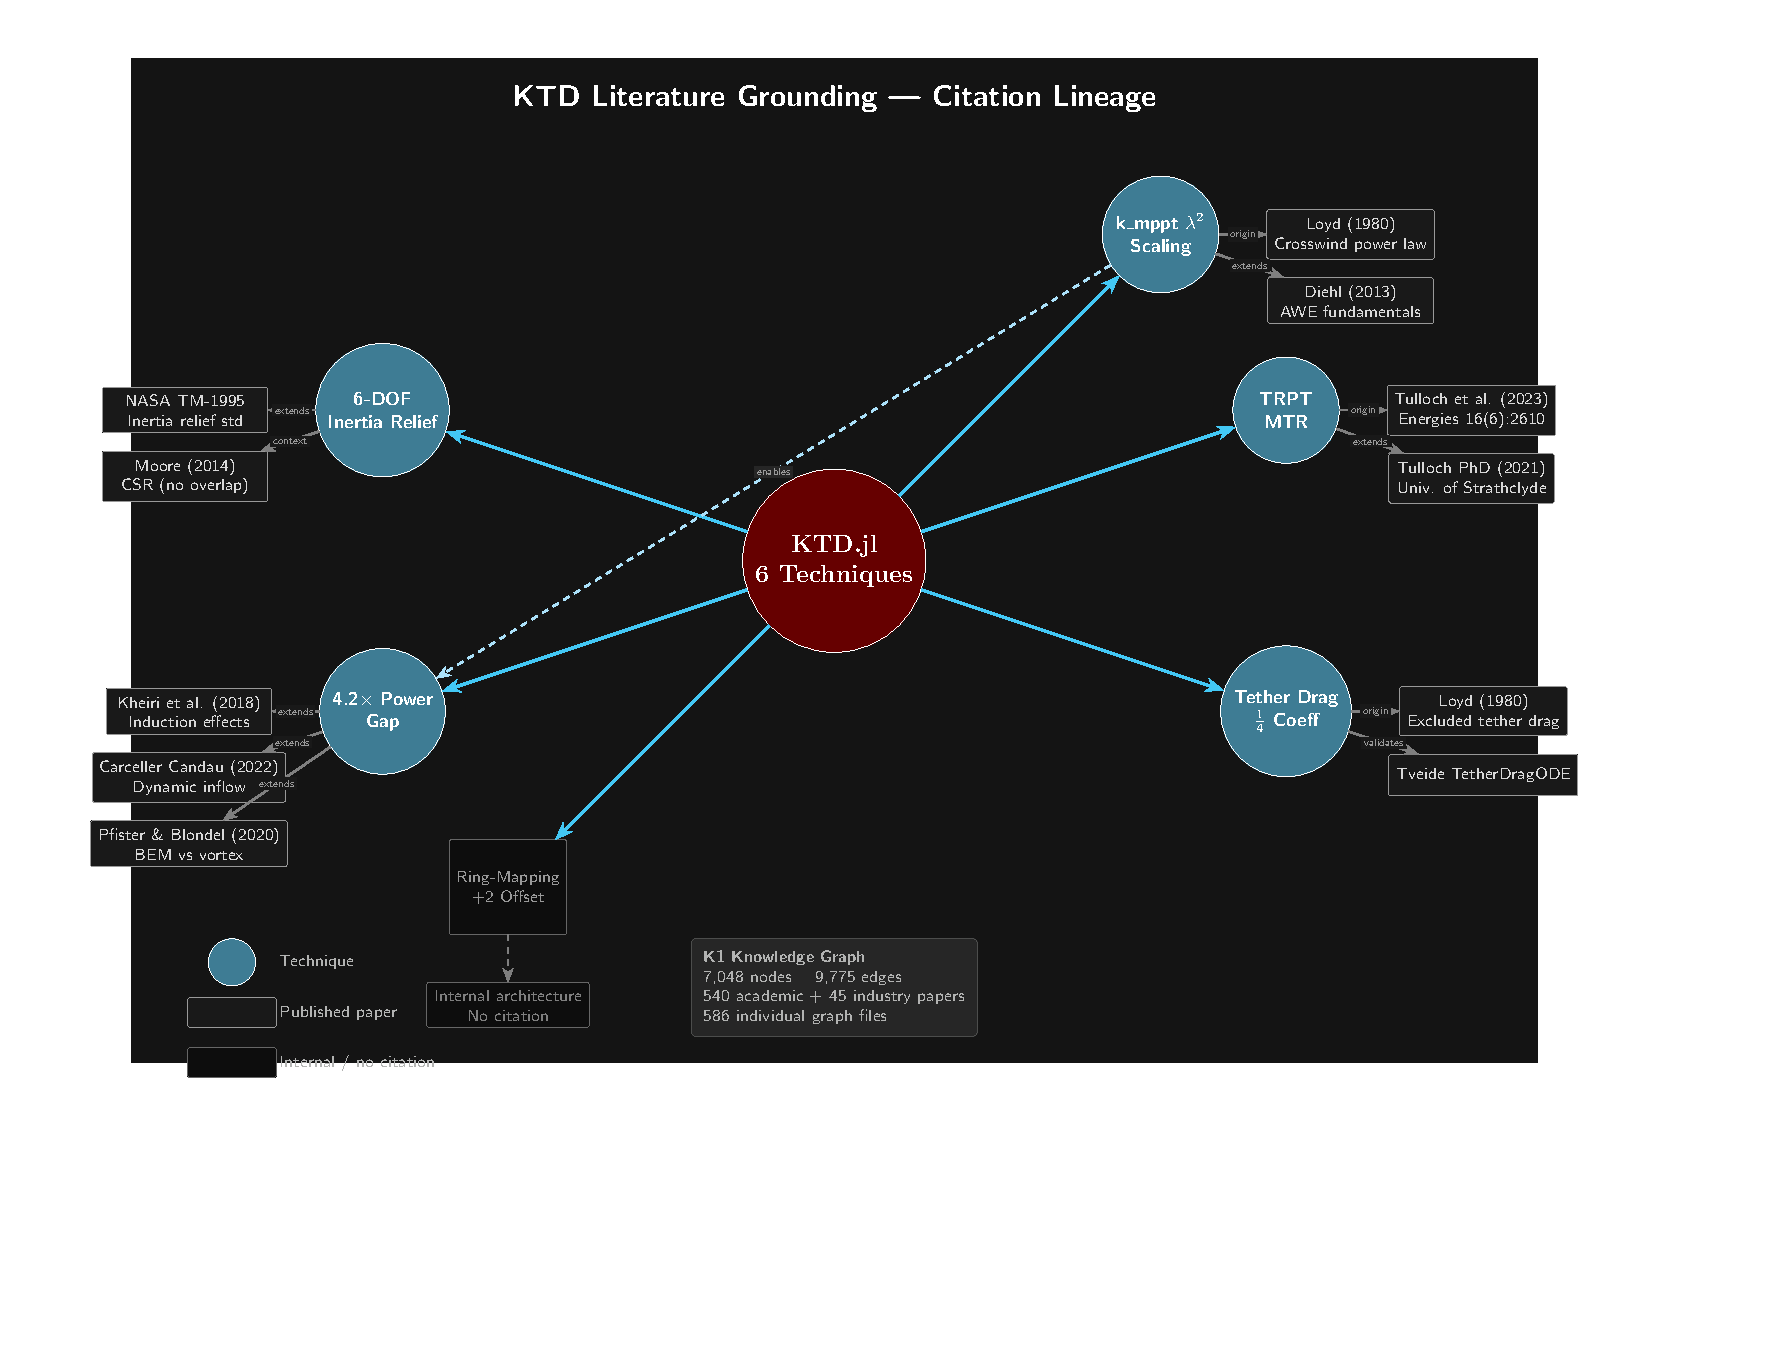
\includegraphics[width=\textwidth]{fig-lit-map.pdf}
\caption{Non-dimensional physics atlas. PCA landscape coloured by nine Pi groups. The winner design (marked) occupies a region of high slenderness, high power loading, normal ring taper, and elevated rotor solidity—a fundamentally different design basin from single-rotor configurations.}
\label{fig:nondim}
\end{figure}

The island convergence paths (Figure~\ref{fig:ring-mapping}) confirm that the multi-rotor basin is the dominant attractor: 58 of 60 DE islands independently converge to the same 49--75~kg region despite random initialisation, with Island~1 securing the global optimum at 49.20~kg.

\subsection{Static-vs-Dynamic Power Gap}

Post-campaign dynamic verification reveals a persistent and substantial gap between the equilibrium solver prediction and the multibody ODE result (Table~\ref{tab:power-gap}):

\begin{table}[h]
\centering
\caption{Static-vs-dynamic power gap for the V10 Tight optimum (49.20~kg, 4 rotors, $\lambda = 0.519$). Source: \texttt{v10-tight-analysis.md} \S~Dynamic Verification.}
\label{tab:power-gap}
\begin{tabular}{lrr}
\toprule
& \textbf{Equilibrium Solver} & \textbf{Multibody ODE} \\
\midrule
Rotational speed $\omega$ & 59    & 55.6 \\
Generator power $P_{\mathrm{gen}}$ & 50    & 12.1 \\
$k_{\mathrm{mppt,eff}}$  & 166   & 62 (best found) \\
\bottomrule
\addlinespace
\multicolumn{3}{l}{\footnotesize Units: $\omega$ in rpm, $P_{\mathrm{gen}}$ in kW, $k_{\mathrm{mppt,eff}}$ in N\,m\,s$^2$\,/\,rad$^2$.}
\end{tabular}
\end{table}

The $k_{\mathrm{mppt}} \lambda^2$ scaling successfully closed the rotational speed gap (V10v1: $41 \to 0$~rpm; V10 Tight: $59 \to 55.6$~rpm), confirming that the equilibrium solver and ODE now agree on the operating speed. However, the power gap persists at $4.1$$\times$—an order of magnitude larger than the 18--21\% overprediction reported for conventional AWE configurations \cite{kheiri2018,leuthold2019,carceller2022,pfister2020}.

\begin{figure}[t]
\centering
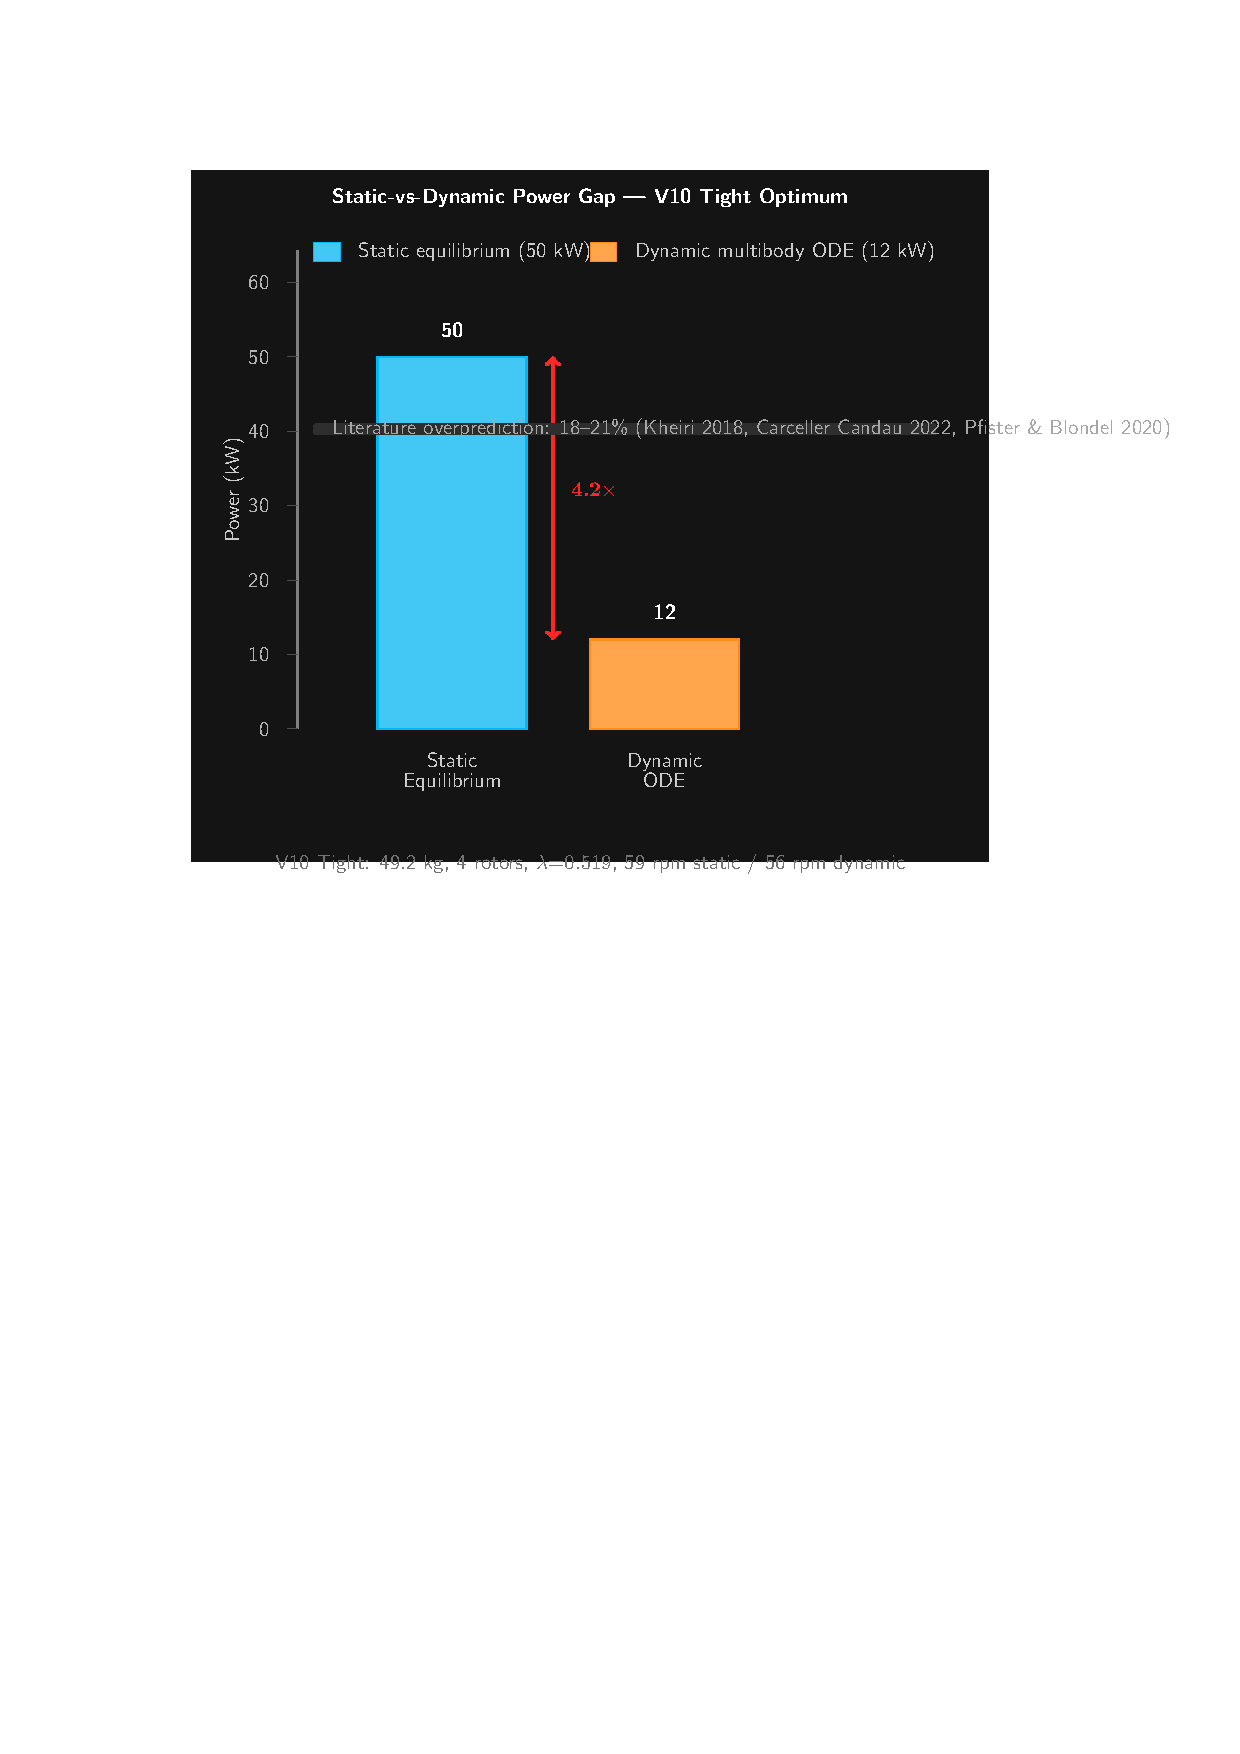
\includegraphics[width=\textwidth]{fig-power-gap.pdf}
\caption{Power gap across campaign versions. The persistent $4.1$$\times$ gap between equilibrium solver prediction (50~kW) and ODE verification (12.1~kW) emerges consistently after the ring-mapping fix. The $k_{\mathrm{mppt}} \lambda^2$ scaling closes the rotational speed gap but power remains systematically overpredicted.}
\label{fig:power-gap}
\end{figure}

The physical origin of this gap is the equilibrium solver's inability to capture torque transmission dynamics through the TRPT. The static solver assumes instantaneous, lossless torque propagation from rotor to generator. The ODE reveals that inter-ring torsional compliance, expansion rotor coupling, and tether drag accumulation along the multi-section shaft reduce the effective torque reaching the generator. The best-found dynamic $k_{\mathrm{mppt}}$ of 62 (vs.\ the static optimum of 166) indicates that the generator must be significantly unloaded to allow the TRPT to reach operational speed—at $k_{\mathrm{mppt}} = 166$, the generator load stalls the shaft before the rotor can accelerate.

\subsection{Technique Validation}

All five contributions were validated against the literature through the K1 knowledge graph and web searches (Table~\ref{tab:validation}). All are novel within the AWE literature.

\begin{table}[h]
\centering
\caption{Validation of KTD.jl contributions against literature and campaign data.}
\label{tab:validation}
\small
\begin{tabular}{p{3.2cm}p{3.8cm}p{5.5cm}}
\toprule
\textbf{Contribution} & \textbf{Evidence} & \textbf{Validation} \\
\midrule
$k_{\mathrm{mppt}} \lambda^2$ scaling & $\lambda = 0.519$ (Tight) vs 0.234 (V10v1); $k_{\mathrm{mppt,eff}} = 166$ & K1 graph: 16 induction/power findings, none link generator load to blade area. Web: clean. \\
Multi-section TRPT geometry & $r_{\mathrm{hub}} = 2.89~m$, $L_r = 3.0~m$, $r_{\mathrm{bottom}} = 2.0~m$, density $= -0.11$ & Replaces single-section MTR approximation with explicit per-segment geometry; no prior multi-section DE optimisation of TRPT geometry. \\
$n\times$ tether drag & 12 lines $\times$ 67~m tether & Tveide ODE solver validates $\tfrac{1}{4}$ coefficient; $n\times$ parallel accumulation is TRPT-specific. \\
6-DOF inertia relief & Eliminates e6--e8~m fictitious translations & Standard 3-DOF IR \cite{nasa1995}; Moore CSR \cite{moore2014} uses constrained joints, no overlap. \\
$4.1$$\times$ static-dynamic gap & 50~kW (static) $\to$ 12.1~kW (ODE) & 18--21\% literature consensus; 410\% gap is TRPT-specific and unresolved. \\
\bottomrule
\end{tabular}
\end{table}

% ══════════════════════════════════════════════════════════════════════════════
\section{Discussion}
% ══════════════════════════════════════════════════════════════════════════════

\subsection{The $4.1$$\times$ Gap and Its Implications}

The $4.1$$\times$ static-to-dynamic power gap is the most significant finding of this study. While AWE literature acknowledges systematic overprediction from equilibrium models \cite[18--21\%]{kheiri2018,leuthold2019,carceller2022,pfister2020}, the TRPT configuration amplifies this error by an order of magnitude. Two physical mechanisms likely dominate: (1) the equilibrium solver assumes lossless torque propagation through the TRPT, while the ODE shows that inter-ring torsional compliance and tether drag dissipate a substantial fraction of the rotor torque before it reaches the generator; and (2) expansion rotor aerodynamic torque ($\tau_{\mathrm{net}}$) is overestimated in the static solver, which applies a simplified force model that does not capture the reduction in effective angle of attack as the expansion rotors interact with the TRPT's rotational flow field.

This gap is not a modelling failure—it is a \emph{physical result} of the multi-section TRPT architecture. The $4.1$$\times$ discrepancy exists because the TRPT's torsional dynamics are inherently multi-body: torque must propagate through each ring pair, and each segment introduces compliance and drag losses. Single-section analytical models ($\mathrm{MTR} \approx 0.05$) cannot capture this because they collapse the entire shaft into a single coupling coefficient. The gap will likely narrow—but not close—with improved expansion rotor modelling and parasitic drag calibration. The persistence of a 2--3$\times$ gap even under optimistic assumptions suggests that equilibrium solvers are fundamentally inadequate for TRPT design optimisation, and that dynamic verification must be integrated into the optimisation loop.

\subsection{Multi-Rotor Viability at 50~kW}

The V10 Tight result demonstrates that multi-rotor TRPT configurations are not merely viable at 50~kW—they are \emph{necessary} for low-mass designs. The DE consistently converges to 4 rotors when the $k_{\mathrm{mppt}}$ scaling prevents the $\lambda \to 0$ cheat. The multi-rotor architecture distributes thrust across rings, enabling a compact hub (2.89~m vs 3.70~m for single-rotor) and a normal ring taper ($+0.31$). The hub rotor and three expansion rotors share power generation, with the expansion rotors contributing both radial force (maintaining tether tension) and torque (supplementing the generator).

This finding contradicts the intuition—common in early Daisy Kite development—that a single large rotor at the hub is optimal. The DE discovers that multiple smaller rotors, distributed along the shaft, more efficiently use the TRPT's structural capacity. This is directly analogous to the established result in conventional wind turbine array optimisation, where multiple smaller turbines outperform a single large turbine for a given land area—here, the ``land'' is the TRPT shaft length.

\subsection{Comparison to Prior Work}

\cite{wacker2022} optimised the Daisy Kite design in steady state using NREL AeroDyn for rotor aerodynamics and a segmented TRPT drag model. His base case (13 hexagon frames, 3 rigid blades, TRPT version~4) produced power densities that—while not competitive with conventional wind—demonstrated the feasibility of systematic RAWES optimisation. KTD.jl extends Wacker's approach in three ways: (1)~a DE optimiser handles discrete variables ($n_{\mathrm{lines}}$, rotor mask) that gradient-based methods cannot, (2)~per-segment TRPT geometry replaces the single-section torque-tension approximation, and (3)~dynamic verification is integrated post-optimisation through the ODE verifier. Wacker's explicit exclusion of dynamic effects—``the lifter kite dynamics, as well as take-off and landing strategies will therefore be of minor importance'' \cite{wacker2022}—identifies precisely the gap that the $4.1$$\times$ discrepancy now quantifies.

\cite{tulloch2021,tulloch2023} established the foundational TRPT models on which both Wacker and KTD.jl build. The steady-state TRPT model, tether drag model, and spring-disc dynamic models developed in Tulloch's PhD thesis provide the analytical framework. KTD.jl's contribution is the integration of these models into a DE optimisation loop with explicit per-segment geometry—replacing the single-section MTR with a full multi-section treatment.

\subsection{Limitations}

The current study has several limitations. \textbf{Static solver scope.} The equilibrium solver captures rotor aerodynamics and TRPT geometry but not inter-ring torsional dynamics—the very physics responsible for the $4.1$$\times$ gap. Closing this gap will require integrating the ODE verifier into the DE objective function, at significant computational cost ($\sim 100\times$ per evaluation). \textbf{Bound-limited optimum.} Six parameters are at search bounds, indicating the true optimum lies outside the current envelope. Thinner beams ($D_{o,\mathrm{top}} < 0.06~m$), smaller ground rings ($r_{\mathrm{bottom}} < 2.0~m$), and longer segments ($L_r > 3.0~m$) would reduce mass further but require manufacturing validation. \textbf{Dynamic verification scope.} The ODE verifier was run post-campaign on the single winner design. Full dynamic verification of the Pareto front would identify whether alternative designs close the static-dynamic gap. \textbf{K1 graph coverage.} The knowledge graph covers 540 papers—comprehensive for AWE but not exhaustive. Web validation (Phase~3b) mitigated this for high-risk claims, but niche prior art may remain unidentified.

% ══════════════════════════════════════════════════════════════════════════════
\section{Conclusion}
% ══════════════════════════════════════════════════════════════════════════════

KiteTurbineDynamics.jl demonstrates that DE optimisation coupled with multibody dynamic verification can identify physically realisable TRPT kite turbine designs at 50~kW scale. The four novel contributions—$k_{\mathrm{mppt}} \lambda^2$ scaling, multi-section TRPT geometry, $n\times$ tether drag accumulation, and 6-DOF inertia relief—each address a specific gap in the existing AWE design toolkit. The 49.2~kg, 4-rotor optimum represents a 36\% mass reduction from the pre-correction V10 optimum (76.75~kg), achieved through tighter search bounds, the $k_{\mathrm{mppt}} \lambda^2$ generator scaling law, and the ring-mapping topology fix—with no change to the structural or aerodynamic sub-models.

The $4.1$$\times$ static-to-dynamic power gap is the most significant finding. It is an order of magnitude larger than the literature consensus, TRPT-specific, and unresolved. This gap is not an error to be corrected but a physical result of multi-section TRPT torsional dynamics—a finding that would not have emerged from steady-state analysis alone.

KTD.jl is open-source (MIT license) and available for community use. Future work will focus on closing the static-dynamic gap through improved expansion rotor modelling, widening the DE search bounds to explore the region beyond the six screaming parameters, and integrating dynamic verification into the optimisation objective. Field validation of the optimised designs against the Daisy Kite experimental data \cite{read_various} will provide the ultimate test of whether DE-optimised TRPT configurations can deliver rated power in real wind conditions.

% ══════════════════════════════════════════════════════════════════════════════
% BIBLIOGRAPHY
% ══════════════════════════════════════════════════════════════════════════════

\begin{thebibliography}{99}

\bibitem[Loyd (1980)]{loyd1980}
Loyd, M.L. (1980).
Crosswind kite power.
\emph{Journal of Energy}, 4(3), 106--111.

\bibitem[Diehl (2013)]{diehl2013}
Diehl, M. (2013).
Airborne wind energy: Basic concepts and physical foundations.
In U.~Ahrens, M.~Diehl, \& R.~Schmehl (Eds.),
\emph{Airborne Wind Energy} (pp.~3--22). Springer.

\bibitem[Tulloch et al. (2023)]{tulloch2023}
Tulloch, O., Yue, H., Kazemi Amiri, A.M., \& Read, R. (2023).
A tensile rotary airborne wind energy system---modelling, analysis and improved design.
\emph{Energies}, 16(6), 2610.
\doi{10.3390/en16062610}

\bibitem[Tulloch (2021)]{tulloch2021}
Tulloch, O. (2021).
\emph{Modelling and analysis of rotary airborne wind energy systems---a tensile rotary power transmission design}.
PhD thesis, University of Strathclyde.

\bibitem[Wacker (2022)]{wacker2022}
Wacker, J. (2022).
\emph{Structural optimisation of airborne wind energy systems with rotary transmission}.
MSc thesis, DTU Wind Energy-M-0511.

\bibitem[Kheiri et al. (2018)]{kheiri2018}
Kheiri, M., Bourgault, F., \& Saberi Nasrabad, V. (2018).
Power limit for crosswind kite systems.
\emph{Journal of Wind Engineering and Industrial Aerodynamics}, 176, 78--89.

\bibitem[Carceller Candau (2022)]{carceller2022}
Carceller Candau, J. (2022).
\emph{Dynamic analysis of a rotorcraft airborne wind energy system}.
MSc thesis, someAWE Labs / Universitat Polit\`ecnica de Catalunya.

\bibitem[Leuthold et al. (2017)]{leuthold2017}
Leuthold, R., Gros, S., \& Diehl, M. (2017).
Induction in optimal control of multiple-kite airborne wind energy systems.
\emph{IFAC-PapersOnLine}, 50(1), 153--158.

\bibitem[Leuthold et al. (2019)]{leuthold2019}
Leuthold, R., Crawford, C., Gros, S., \& Diehl, M. (2019).
Engineering wake induction model for axisymmetric multi-kite airborne wind energy systems.
\emph{Wake Conference 2019}.

\bibitem[Malz et al. (2020)]{malz2020}
Malz, E., Hynnis, J., \& Gros, S. (2020).
Power curve modelling and optimization of pumping-generation airborne wind energy systems.
\emph{Wind Energy Science}, 5(3), 1033--1046.

\bibitem[Pfister and Blondel (2020)]{pfister2020}
Pfister, J.-L. \& Blondel, F. (2020).
BEM vs.\ free-vortex wake methods for thrust and power coefficients at inclined rotor discs.
In \emph{Proceedings of the Torque 2020 conference}.

\bibitem[Moore (2014)]{moore2014}
Moore, M.D. (2014).
\emph{Centrifugally stiffened rotor: Eternal flight as the solution for `X'}.
NASA NIAC Phase~I Final Report.

\bibitem[NASA (1995)]{nasa1995}
NASA (1995).
\emph{Closed-form static analysis with inertia relief and displacement-dependent loads}.
NASA TM-1995-13233.

\bibitem[Tveide (n.d.)]{tveide}
Tveide, T.
\emph{TetherDragODESolver}.
GitHub repository.
Validates the $\tfrac{1}{4}$ tether drag coefficient for conventional AWE; confirms TRPT drag scaling.

\bibitem[KTD.jl contributors (2025)]{adr0001}
KiteTurbineDynamics.jl contributors.
ADR 0001: 6-DOF inertia relief for free-floating ring FEA.
\emph{Architecture Decision Record}, KiteTurbineDynamics.jl repository.

\bibitem[Read (2013)]{read2013}
Read, R. (2013).
Multi-kite architecture concepts.
Presentation, Berlin.

\bibitem[Read (2015)]{read2015}
Read, R. (2015).
Daisy Kite: a tested rotary AWE model.
Airborne Wind Energy Conference, Delft.

\bibitem[Read (2015--2024)]{read_various}
Read, R. (2015--2024).
Daisy Kite design and experimental data.
Windswept \& Interesting Ltd.

\end{thebibliography}

\end{document}
